% ARFC Team: Some good examples of how to use beamer are in this file.
% You can use this to guide the preparation of slides.

\begin{frame}
  \frametitle{Columns}
  % a comment
        \begin{columns}
                \column[t]{5cm}
                Sometimes things need to be put side by side, in two nice
                looking columns.

                Maybe one column involves a quotation.

                \begin{quote}
                        Explicit is better than implicit. -- The Zen of Python
                \end{quote}


                And, also, perhaps, a logo.
                \begin{center}
                        
\includegraphics[height=0.2\textheight]{./images/arfc-logo}
                \end{center}
                \column[t]{5cm}
        \begin{figure}[htbp!]
        \begin{center}
      
\includegraphics[height=4cm]{./images/kitten}
    \end{center}
          \caption{A caption describing the image. \cite{lastname_firstword_1900}.}
    \label{fig:kittenfigure}
  \end{figure}
        \end{columns}
\end{frame}

\begin{frame}[fragile]
  \frametitle{Some Code}
        I have to use the fragile syntax for code slides.
        \begin{minted}{python}
def meow(volume):
    """Make a demanding noise at the specified volume

    Parameters
    ----------
    volume: int
        The volume of the demand. No relation to importance.

    Returns
    -------
    str
        meow
    """
    o = 'o'*volume
    return 'me'+ o + 'ow'
\end{minted}
\end{frame}
\begin{frame}
  \frametitle{An Image}
  % a comment
  \begin{figure}[htbp!]
    \begin{center}
      
\includegraphics[height=4cm]{./images/kitten}
    \end{center}
          \caption{A caption describing the image. \cite{lastname_firstword_1900}.}
    \label{fig:kittenfigure}
  \end{figure}
\end{frame}

\begin{frame}
  \frametitle{A Table}
        Frames (slides) can have ``blocks.''
        \begin{block}{This one is about a cat}
                A cat in a hat.
        \end{block}
        \begin{block}{A cat}
                In a hat.

                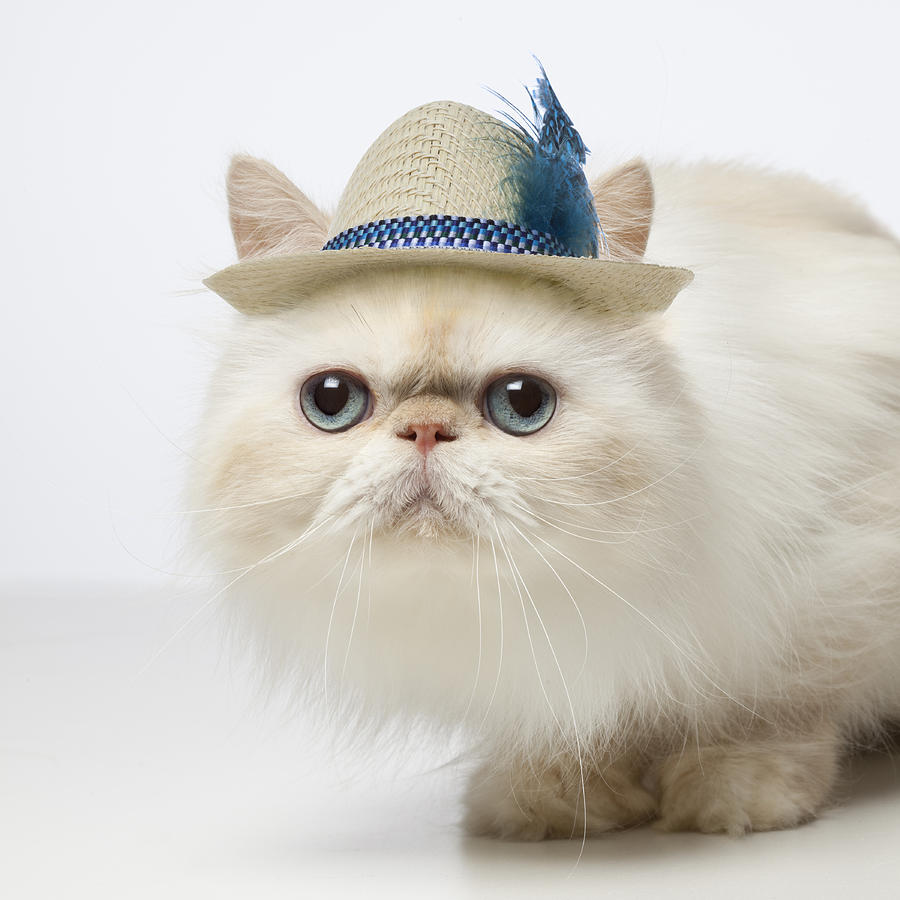
\includegraphics[height=0.2\textheight]{./images/catinhat}
        \end{block}

\end{frame}
\begin{frame}
  \frametitle{Cat Math: Part 1}
  % a comment
        \begin{align}
                x &= y
                \intertext{where}
                x &= \mbox{cats}\\
                y &= \mbox{peculiar}
        \end{align}
\end{frame}

\begin{frame}
\frametitle{Cat Math: Part 2}
        Everything in Beamer is just like in \LaTeX.
        Right down to the theorems.
        \begin{theorem}[Pythagoras]
                $ a^2 + b^2 = c^2$
        \end{theorem}
        \begin{corollary}
                $ x + y = y + x  $
        \end{corollary}
        \begin{proof}
                $\omega +\phi = \epsilon $
        \end{proof}

\end{frame}

\begin{frame}
  \frametitle{Blue and Orange are Fierce}
  % a comment
        Those are the Illini Colors. Use them like you see them in Figure
        \ref{fig:fierce}.
  \begin{figure}[htbp!]
    \begin{center}
      
\includegraphics[height=4cm]{./images/fierce}
    \end{center}
          \caption{Kristofer Hivju is pretty serious about this color palette \cite{lastname_firstword_1900}.}
    \label{fig:fierce}
  \end{figure}
\end{frame}

\begin{frame}
        \frametitle{Table}
           % Future Fuel Cycles
    \begin{table}
      \centering
      \footnotesize{
      \begin{tabular}{|l|l|l|}
        \multicolumn{3}{c}{\textbf{Domestic Fuel Cycle Options}}\\
        \hline
        Title & Description& Challenges \\
        \hline
        \hline
        Open          & Once Through         & High Temperatures, Volumes \\
                      & Current US PWR Fleet &      \\
                      & No Separations       &      \\
                      & No Recycling         &      \\
                      & Higher Burnups &      \\
        \hline
        Modified Open & Partial Recycling     & Both high volumes \\
                      & Next Gen. PWR Fleet   &   and variable spent fuel streams \\
                      & Limited Separations   &      \\
                      & Limited Transmutation &      \\
                      & Advanced Fuel Forms   &      \\
                      & HLW treatment         &      \\
        \hline
        Closed        & Full Recycling       & Variable spent fuel streams \\
                      & Full Separations &      \\
                      & Full Recycling &      \\
                      & VHTGR, SFRs, &      \\
                      & other transmutation & \\
                      & HLW treatment  &      \\
        \hline
      \end{tabular}
      \caption[Fuel Cycle Options]{Domestic Fuel Cycle Options }
      \label{tab:fco}
      }
    \end{table}

\end{frame}
